\documentclass[a4paper]{article} 
\usepackage{geometry,fancyhdr,caption,subcaption,graphicx,psfrag,amsfonts,textcomp,mathtools,amsmath,hyperref} 

% settings courtesy of http://www.tjansson.dk/?p=419
\usepackage{listings}
\usepackage{color}
\usepackage{textcomp}
\definecolor{listinggray}{gray}{0.9}
\definecolor{lbcolor}{rgb}{0.9,0.9,0.9}
\lstset{
	backgroundcolor=\color{lbcolor},
	tabsize=4,
	rulecolor=,
	language=matlab,
        basicstyle=\scriptsize,
        upquote=true,
        aboveskip={1.5\baselineskip},
        columns=fixed,
        showstringspaces=false,
        extendedchars=true,
        breaklines=true,
        prebreak = \raisebox{0ex}[0ex][0ex]{\ensuremath{\hookleftarrow}},
        frame=single,
        showtabs=false,
        showspaces=false,
        showstringspaces=false,
        identifierstyle=\ttfamily,
        keywordstyle=\color[rgb]{0,0,1},
        commentstyle=\color[rgb]{0.133,0.545,0.133},
        stringstyle=\color[rgb]{0.627,0.126,0.941},
}

\title{Mandatory exercise 5 \\
Signal and Image Processing 2012} 
\author{Jens P. Raaby \\
\url{frn617@diku.dk}}

\begin{document} 
\maketitle

\section*{Question 5.1}
In order to implement an edge detector based on maximum gradient magnitude, I used the scale function to calculate horizontal and vertical first derivatives (with slight Gaussian blurring) and then combined them to find the magnitude.

In order to implement the Marr-Hildreth edge detector I altered the simple gradient magnitude version to use the second derivative of Gaussian (DoG) which approximates the Laplacian. The method then determines the zero crossings by comparing all pairs of pixels (vertically and horizontally) to find if they have opposite signs. A threshold is used to allow variable elimination of erroneous edges. 

Both edge detectors are defined in the function edgedetector.m, see appendix \ref{appendix-edgedetector}.

\subsection*{Examples}
In order to find the best parameters for the standard deviation $\sigma$ and threshold parameters, I created a simple GUI with GUIDE. Source code is included in a separate file (it calls the function edgedetector as defined in appendix \ref{appendix-edgedetector}).

The first example is the rice.tif image. This is fairly simple, and both methods yielded good results, shown in figure \ref{fig:rice}. There was not much difference between the methods in this case. Both exhibit some slight discontinuity in the edges towards the lower right (note how the original image gets darker in this corner).
\begin{figure}
    
        \centering
        \begin{subfigure}[b]{0.3\textwidth}
                \centering
                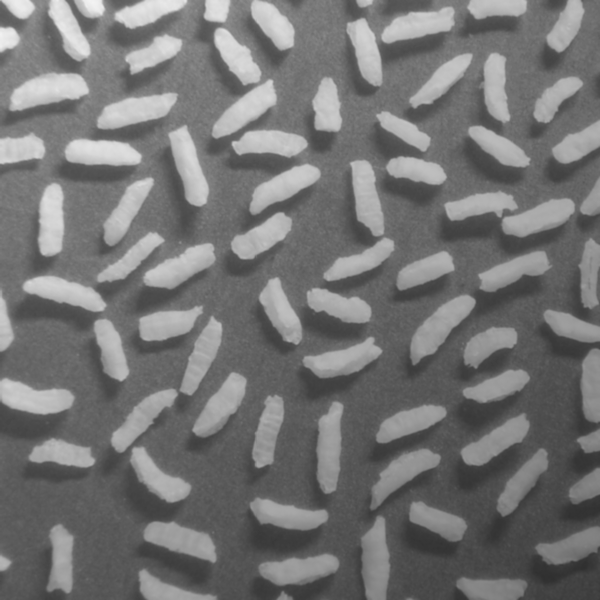
\includegraphics[width=\textwidth]{q1-rice-orig.png}
                \caption{Rice.tif (original)}
                \label{fig:8a}
        \end{subfigure}
        \begin{subfigure}[b]{0.3\textwidth}
                \centering
                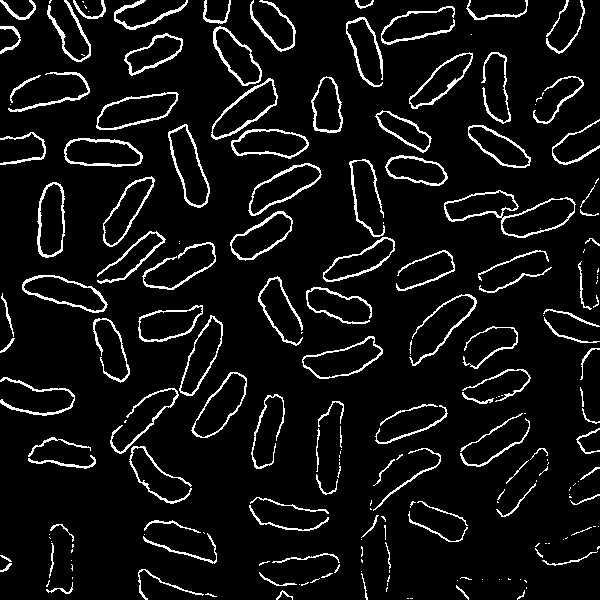
\includegraphics[width=\textwidth]{q1-rice-mag.png}
                \caption{Gradient detector, \\$\sigma (X) = 0.7,  \sigma (Y) = 0.5, \\threshold = 0.3$}
                \label{fig:8b}
                
        \end{subfigure}
        \begin{subfigure}[b]{0.3\textwidth}
                \centering
                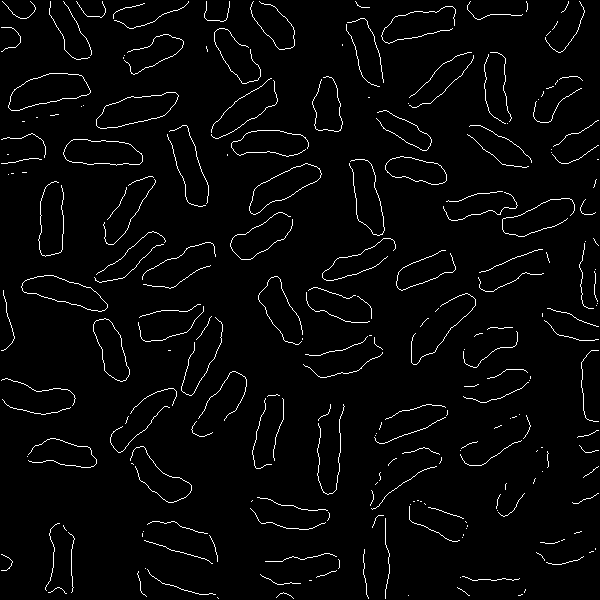
\includegraphics[width=\textwidth]{q1-rice-mh.png}
                \caption{Marr-Hildreth detector, \\$\sigma (X) = 4, \sigma (Y) = 4, \\threshold = 9*10^{-4}$}
                \label{fig:8c}
                
        \end{subfigure}
        
        \caption{Results of finding edges on Rice.tif}        
        \label{fig:rice}
\end{figure}

The second image tested is house.tif. This incorporates a lot of small scale vertical and horizontal edge detail in the form of bricks and roof tiles, and therefore the parameters can be adjusted to see how they affect the edge detection.
With the basic (gradient based) edge detection method, the lines on the roof are detected well, and the outlines of the building seem to be well defined (figure \ref{fig:1b}). The windows are lacking some detail and there are a couple of noisy areas (particularly on the right). One of the motivators for adding a second $\sigma$ parameter for the y-direction was the way in which this image has differing levels of detail in each direction.

Applying Marr-Hildreth results in edges detected with more `connectedness', shown in figure \ref{fig:1c}. The edges are all 1-pixel thick because of the way zero-crossings are detected, so they might not appear as strong as the former method's detected edges. The corners of the building have becomed rounded (this is caused by the Gaussian blurring - the $\sigma$ parameters had to be increased to avoid including too much noise) and don't look very sharp. However, in terms of identifying features this method is better. The roof lines are not as complete as in the previous case, but correcting this for the localised area (by reducing the $\sigma (Y)$ value) adds noise to other areas of the image.
\begin{figure}
    
        \centering
        \begin{subfigure}[b]{0.3\textwidth}
                \centering
                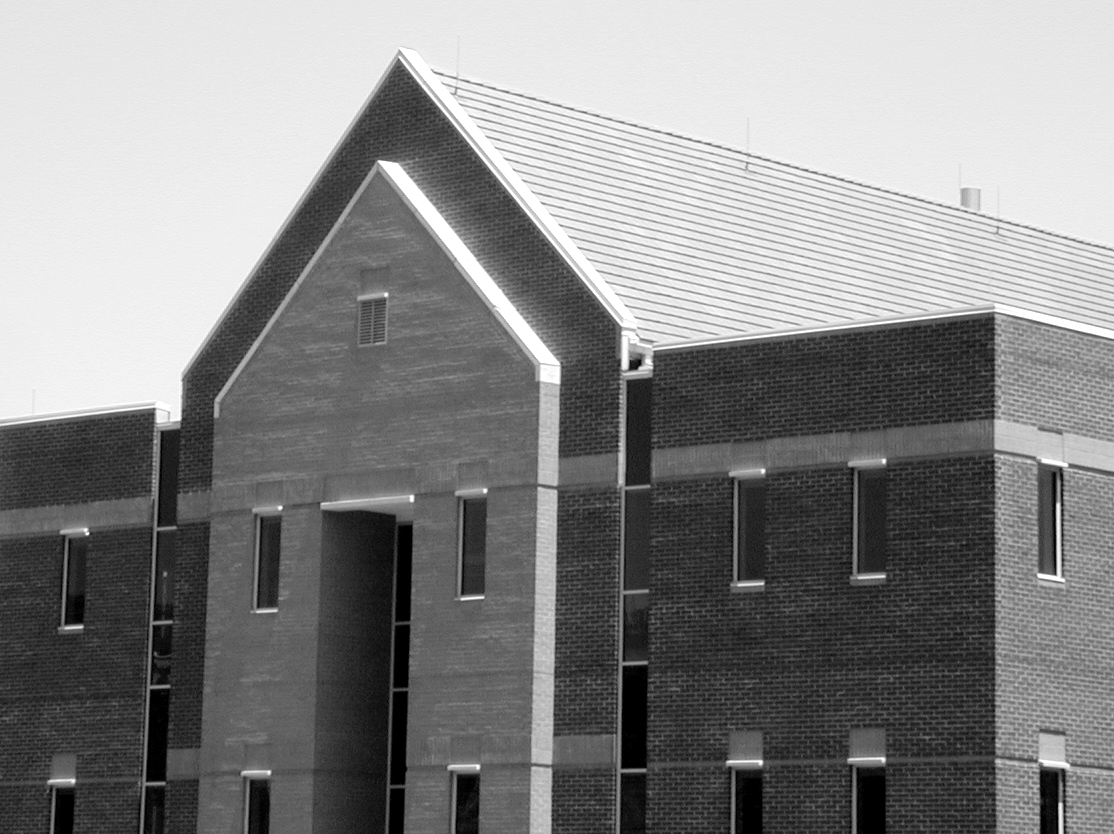
\includegraphics[width=\textwidth]{q1-house-orig.png}
                \caption{House.tif (original)}
                \label{fig:1a}
        \end{subfigure}
        \begin{subfigure}[b]{0.3\textwidth}
                \centering
                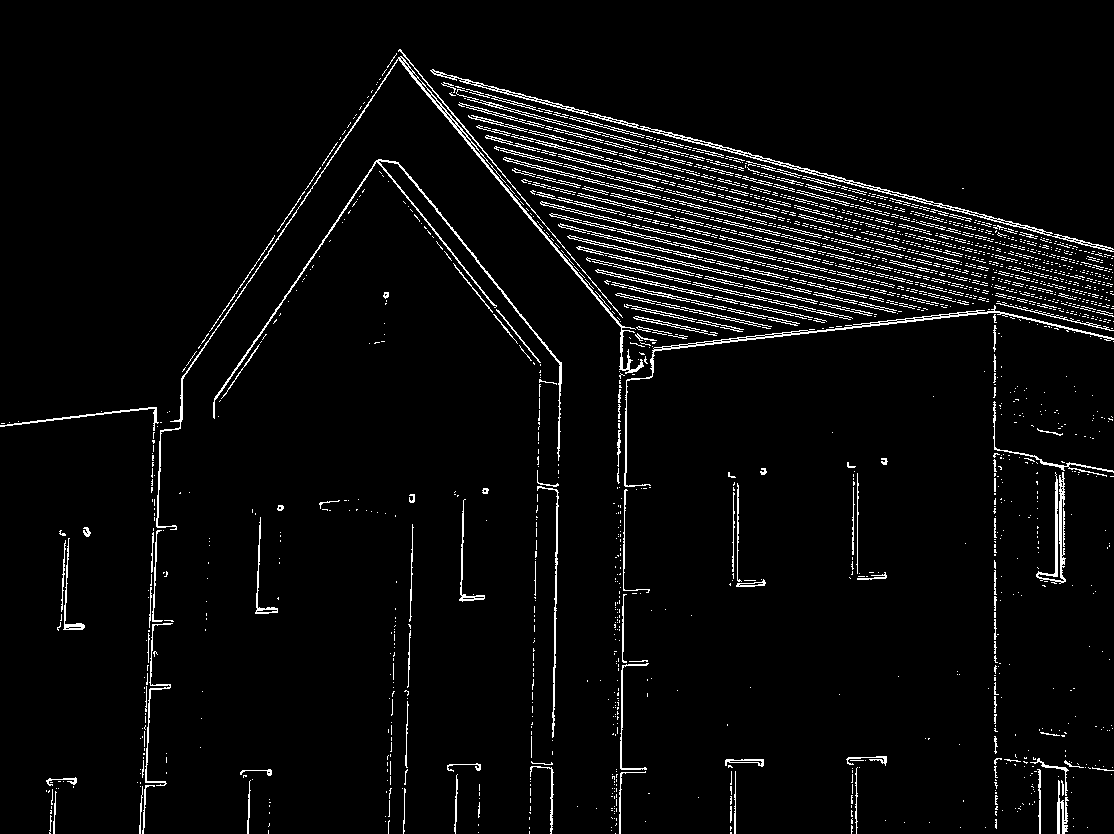
\includegraphics[width=\textwidth]{q1-house-mag.png}
                \caption{Gradient detector, $\sigma (X) = 0.6, \sigma (Y) = 0.7, threshold = 0.3$}
                \label{fig:1b}
                
        \end{subfigure}
        \begin{subfigure}[b]{0.3\textwidth}
                \centering
                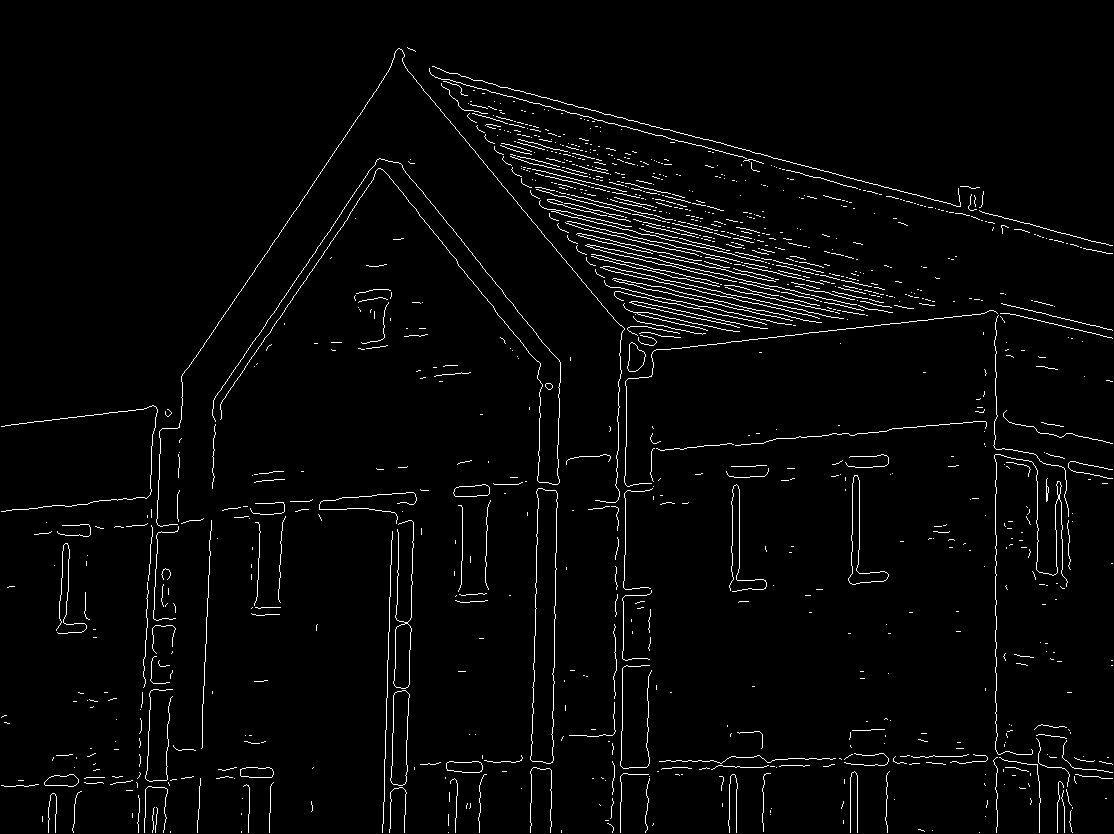
\includegraphics[width=\textwidth]{q1-house-mh.png}
                \caption{Marr-Hildreth detector, $\sigma (X) = 4, \sigma (Y) = 3.8, threshold = 6.5*10^{-4}$}
                \label{fig:1c}
                
        \end{subfigure}
        
        \caption{Results of finding edges on House.tif}        
        \label{fig:1}
\end{figure}

The third test image is Lena. This picture includes smooth areas such as the skin and hat, as well as random (almost fractal) detail in the hair. The results shown in figure \ref{fig:2} show that the simple detector did a fairly good job at detecting edges but left plenty of noise. The Marr-Hildreth result was better in some regards, especially as it created thinner edges.
\begin{figure}
    
        \centering
        \begin{subfigure}[b]{0.3\textwidth}
                \centering
                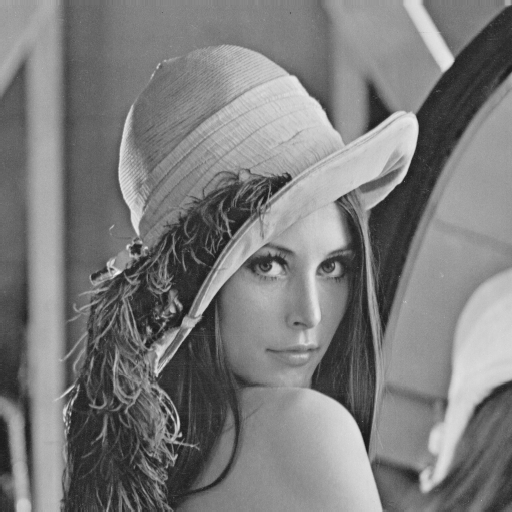
\includegraphics[width=\textwidth]{q1-lena-orig.png}
                \caption{Lena.tif (original)}
                \label{fig:2a}
        \end{subfigure}
        \begin{subfigure}[b]{0.3\textwidth}
                \centering
                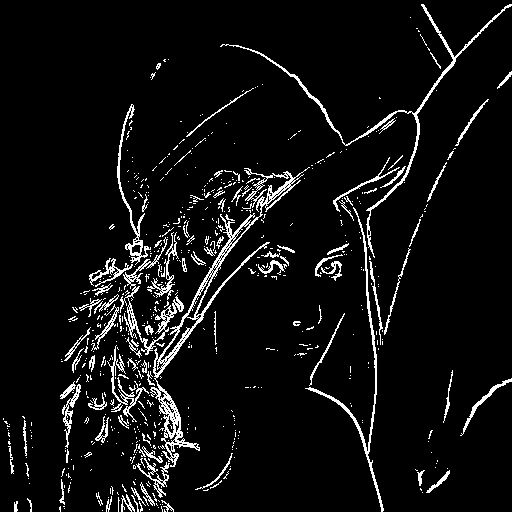
\includegraphics[width=\textwidth]{q1-lena-mag.png}
                \caption{Gradient detector, \\$\sigma (X) = 0.7,  \sigma (Y) = 0.5, \\threshold = 0.2$}
                \label{fig:2b}
                
        \end{subfigure}
        \begin{subfigure}[b]{0.3\textwidth}
                \centering
                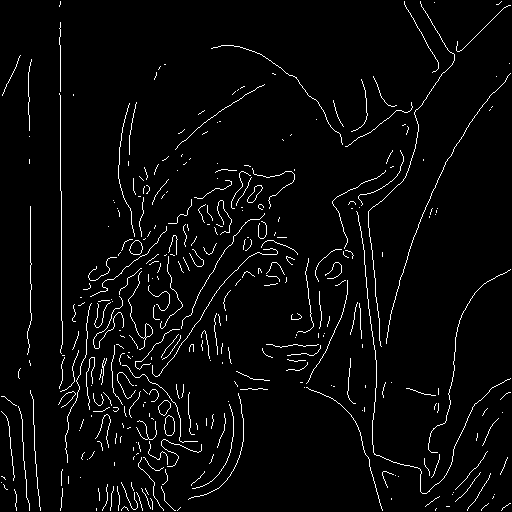
\includegraphics[width=\textwidth]{q1-lena-mh.png}
                \caption{Marr-Hildreth detector, \\$\sigma (X) = 4, \sigma (Y) = 3.8, \\threshold = 6.5*10^{-4}$}
                \label{fig:2c}
                
        \end{subfigure}
        
        \caption{Results of finding edges on Lena.tif}        
        \label{fig:2}
\end{figure}


\clearpage
\section*{Question 5.2 - Canny Edge Detector}
The Canny edge detector is implemented in the file cannydetector.m, see appendix \ref{appendix-cannydetector}. The function is mostly vectorised, apart from the non-maxima suppression which runs through the entire pixel set and compares directional neighbours' gradient magnitudes. This is more elegantly handled in Matlab's own implementation which therefore runs a lot faster.

The sub-function which tries to close loops. $connectivity(strong,weak,directions)$, connects weak edge pixels which are in the same direction as neighbouring strong edge pixels.
It is a little unclear how to implement the behaviour perfectly in the textbook, so I also tried using the Matlab function $bwselect$ which selects pixels which are connected to specified coordinates. That means that an entire line connected to one strong pixel will be created. I include both methods in figure \ref{fig:4}, where it is clear (in particular in the central images \ref{fig:4b} \& \ref{fig:4e}) that the $bwselect$ method picks up more connected edges. In this particular case I did not want the bricks to be included, but the roof tiles were meant to remain. This was most successful using my own method. 

With the other settings, I found the $bwselect$ method tended to pick up unwanted details; though this would most likely be alleviated by raising the lower threshold slightly. In the listing provided in the appendix, I commented out the $bwselect$ method. 

The images of Lena shown in figure \ref{fig:3} were created using my own edge completer. Note that with the lower upper threshold (shown in figure \ref{fig:3c}) a lot of the edges are almost complete, but there is a lot more noise.

\begin{figure}[h]
    
        \centering
        \begin{subfigure}[b]{0.3\textwidth}
                \centering
                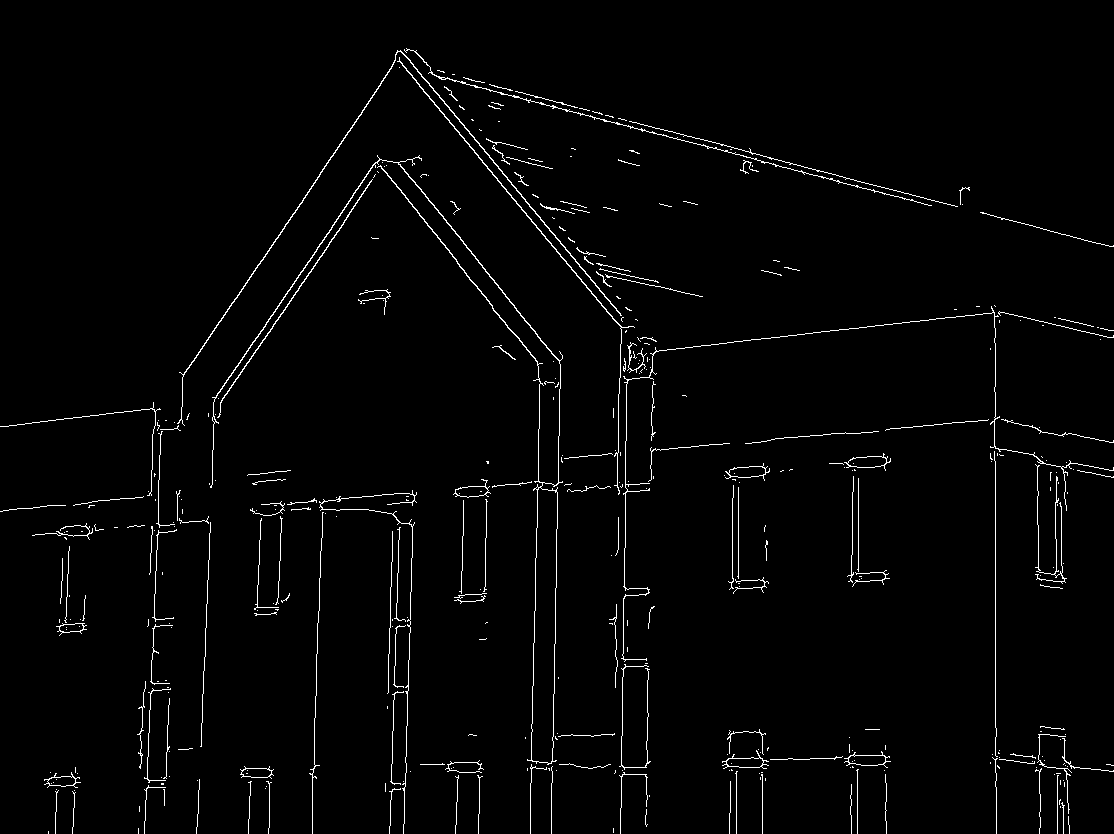
\includegraphics[width=\textwidth]{q2-house-canny-020083.png}
                \caption{$t_{low}=0.08, t_{high}=0.2, \sigma=3$}
                \label{fig:4a}
        \end{subfigure}
        \begin{subfigure}[b]{0.3\textwidth}
                \centering
                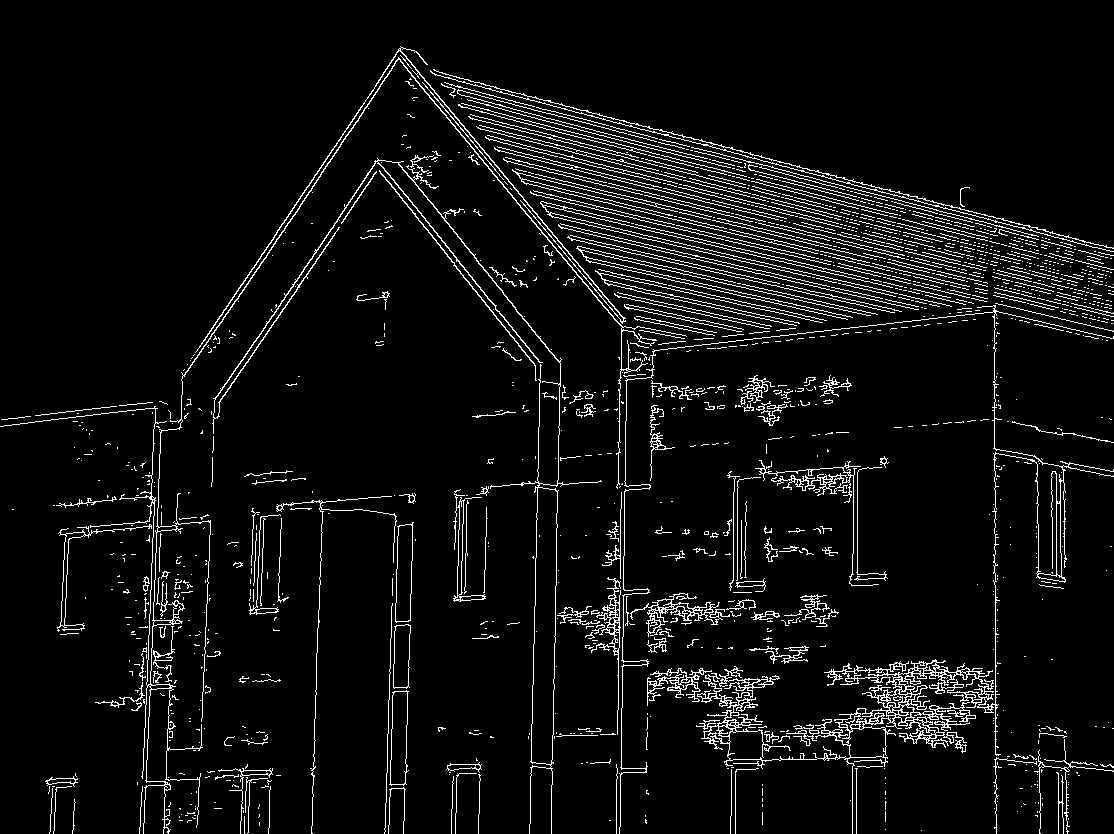
\includegraphics[width=\textwidth]{q2-house-canny-02006rt2.png}
                \caption{$t_{low}=0.06, t_{high}=0.2, \sigma=\sqrt{2}$}
                \label{fig:4b}
                
        \end{subfigure}
        \begin{subfigure}[b]{0.3\textwidth}
                \centering
                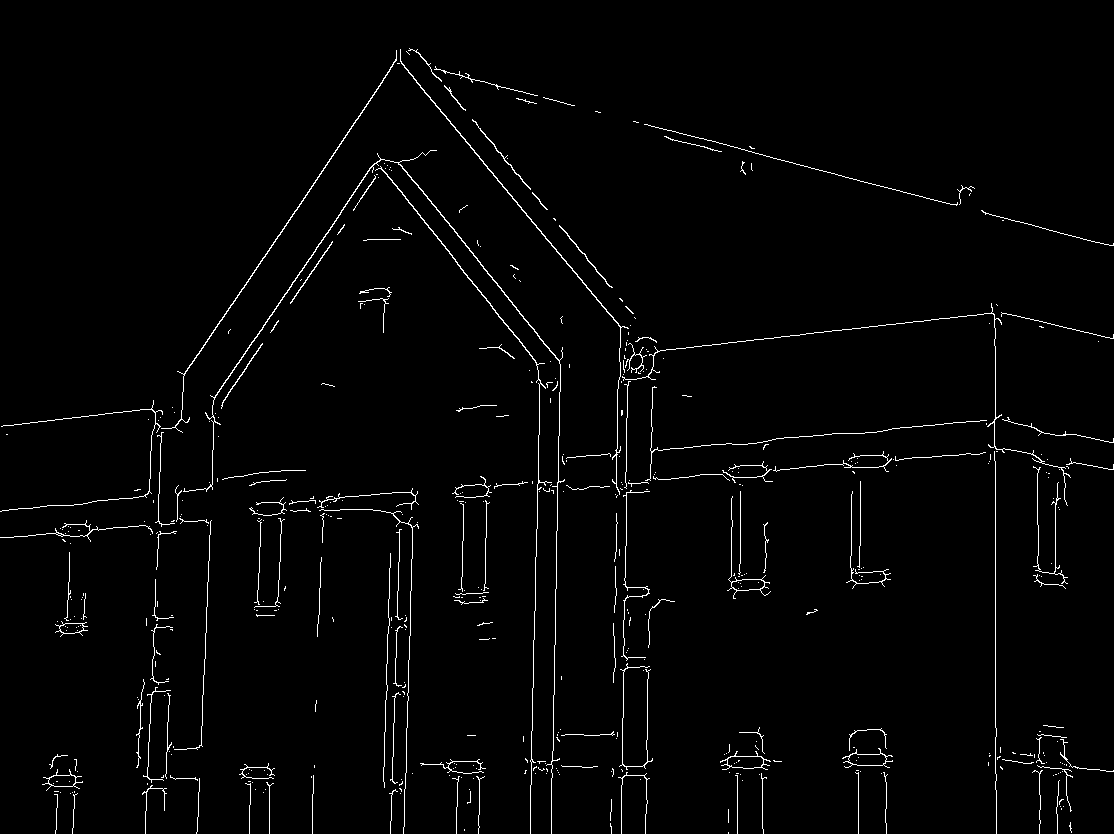
\includegraphics[width=\textwidth]{q2-house-canny-0150063rt2}
                \caption{$t_{low}=0.06, t_{high}=0.15, \sigma=3*\sqrt{2}$}
                \label{fig:4c}
                
        \end{subfigure}
        
        \begin{subfigure}[b]{0.3\textwidth}
                \centering
                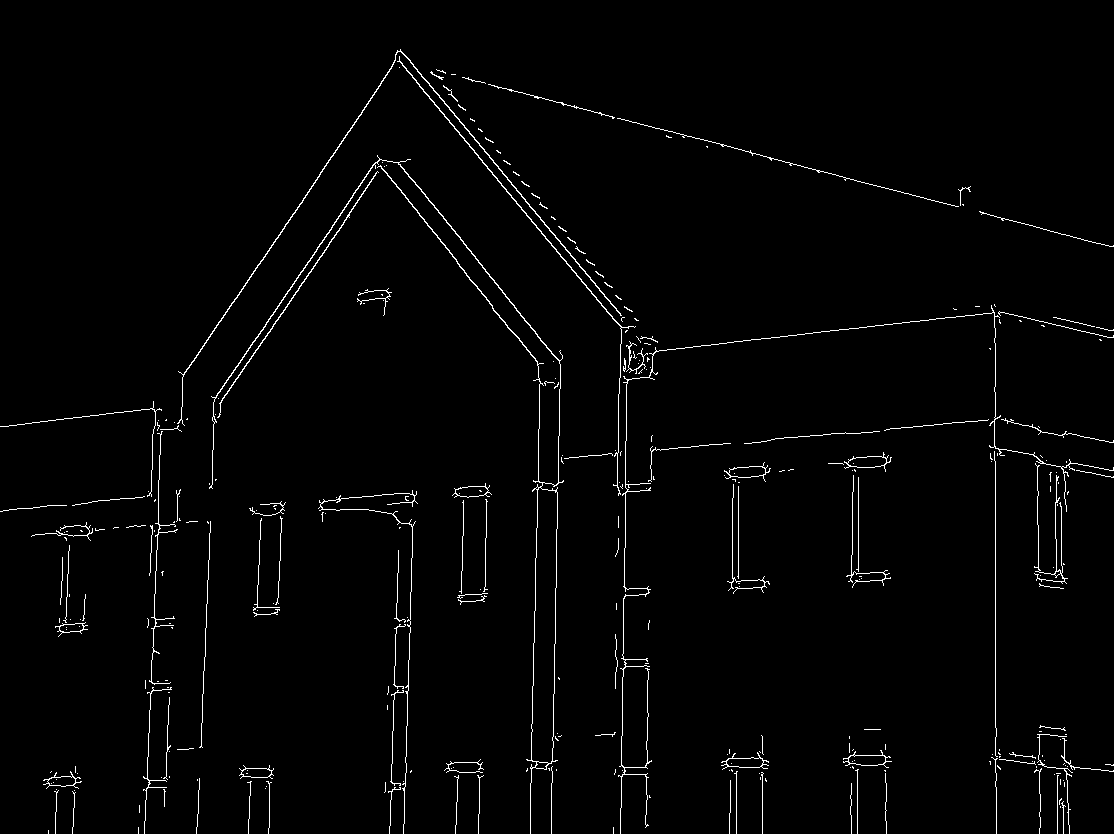
\includegraphics[width=\textwidth]{q2-house-canny-020083-my.png}
                \caption{$t_{low}=0.08, t_{high}=0.2, \sigma=3$}
                \label{fig:4d}
        \end{subfigure}
        \begin{subfigure}[b]{0.3\textwidth}
                \centering
                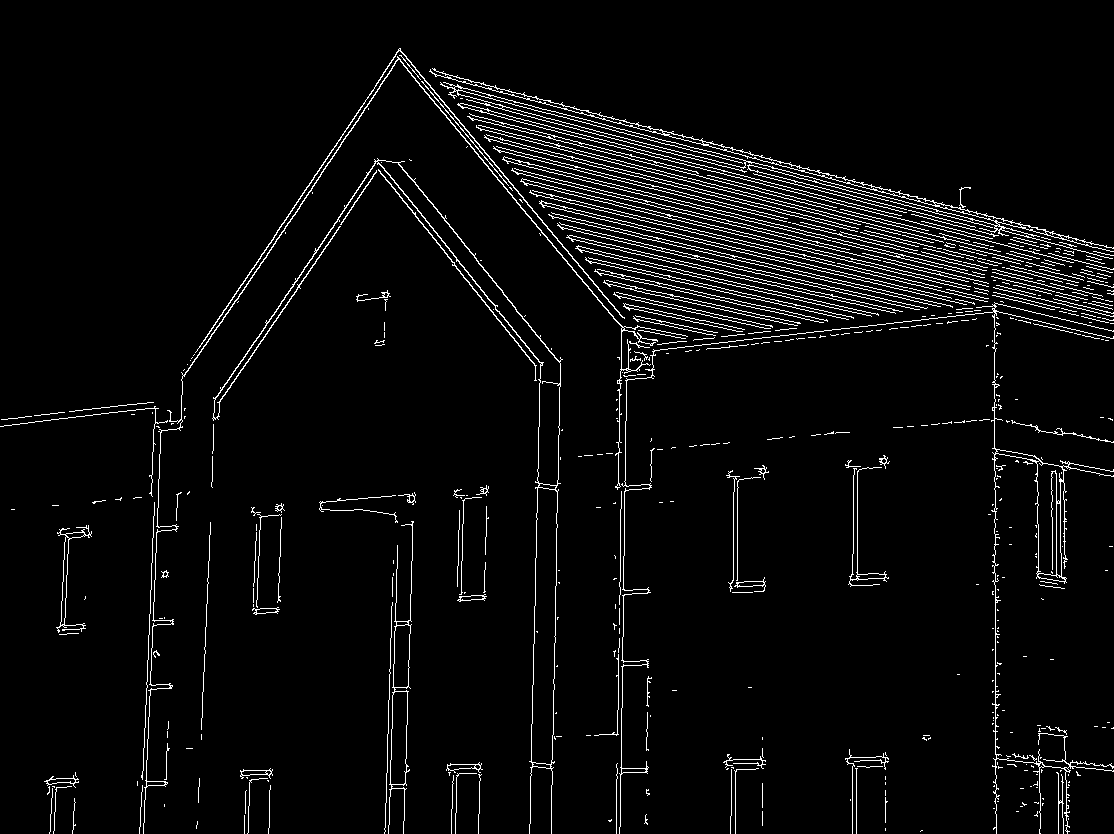
\includegraphics[width=\textwidth]{q2-house-canny-02006rt2-my.png}
                \caption{$t_{low}=0.06, t_{high}=0.2, \sigma=\sqrt{2}$}
                \label{fig:4e}
                
        \end{subfigure}
        \begin{subfigure}[b]{0.3\textwidth}
                \centering
                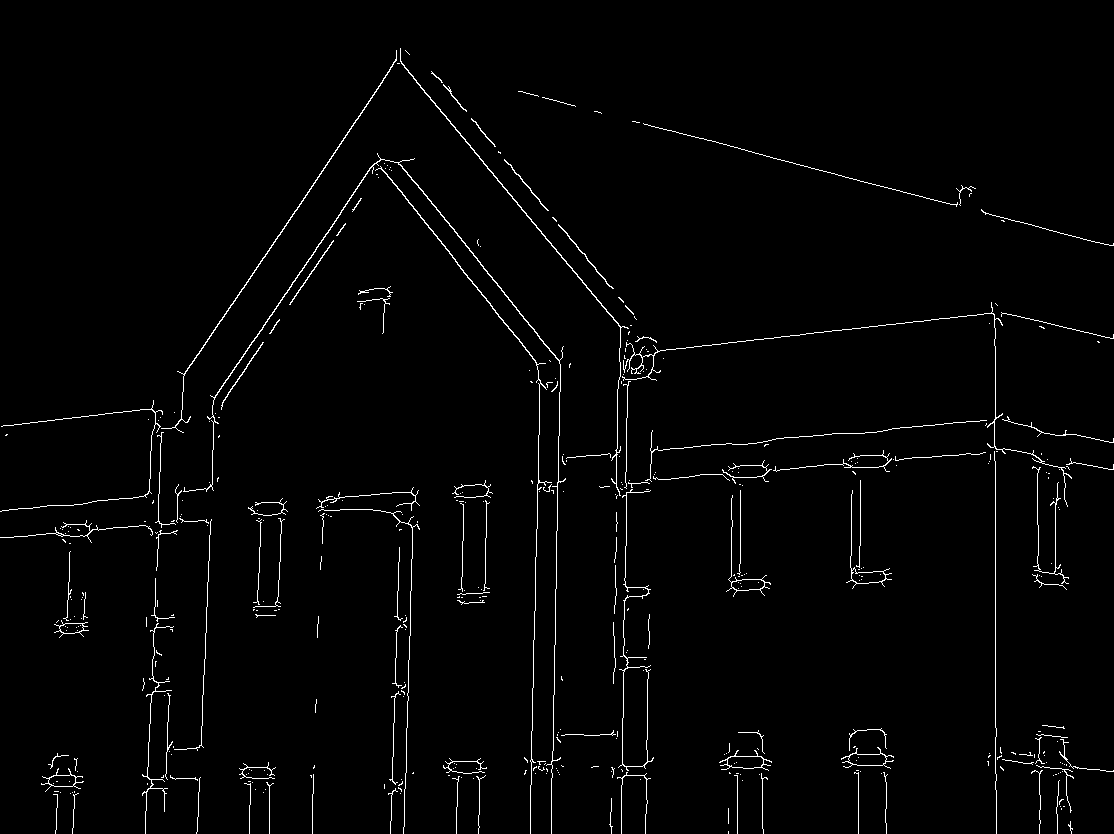
\includegraphics[width=\textwidth]{q2-house-canny-0150063rt2-my.png}
                \caption{$t_{low}=0.06, t_{high}=0.15, \sigma=3*\sqrt{2}$}
                \label{fig:4f}
                
        \end{subfigure}
        
        \caption{Results of Canny edge detection on House.tif.  Upper row using bwselect for connectivity, below using my simpler directional implementation}        
        \label{fig:4}
\end{figure}
\begin{figure}[h]
    
        \centering
        \begin{subfigure}[b]{0.3\textwidth}
                \centering
                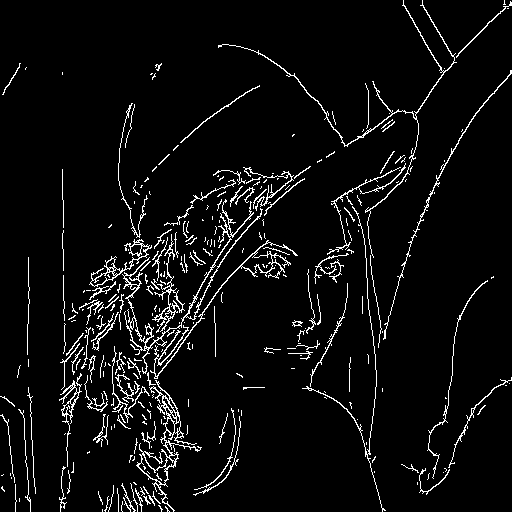
\includegraphics[width=\textwidth]{q2-lena-canny-0200814.png}
                \caption{$t_{low}=0.08, t_{high}=0.2, \sigma=\sqrt{2}$}
                \label{fig:3a}
        \end{subfigure}
        \begin{subfigure}[b]{0.3\textwidth}
                \centering
                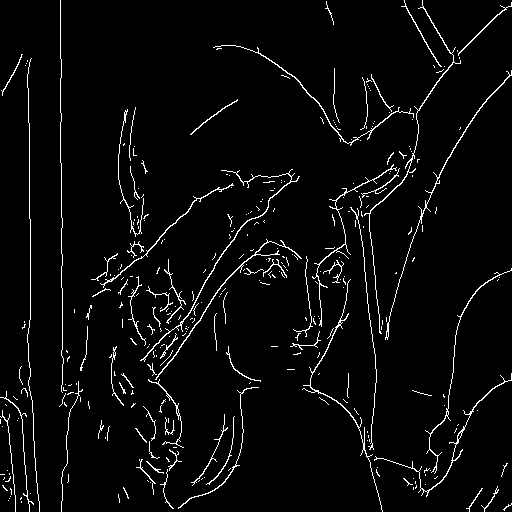
\includegraphics[width=\textwidth]{q2-lena-canny-020084.png}
                \caption{$t_{low}=0.08, t_{high}=0.2, \sigma=4$}
                \label{fig:3b}
                
        \end{subfigure}
        \begin{subfigure}[b]{0.3\textwidth}
                \centering
                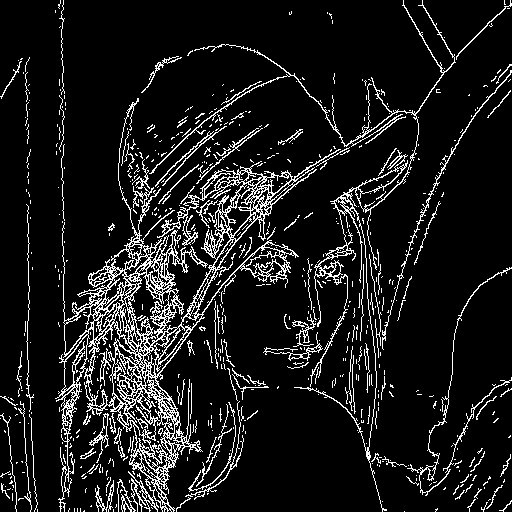
\includegraphics[width=\textwidth]{q2-lena-canny-010081.png}
                \caption{$t_{low}=0.08, t_{high}=0.1, \sigma=1$}
                \label{fig:3c}
                
        \end{subfigure}
        
        \caption{Results of Canny edge detection on Lena.tif}        
        \label{fig:3}
\end{figure}

\clearpage
\section*{Question 5.3}
For the double thresholding I created a function doublethreshold.m, listed in appendix \ref{appendix-doublethreshold}.

The iterative threshold solution was very straightforward to calculate (and realatively fast). However, the double thresholding method varies in speed considerably according to the epsilon value (used to determine the upper threshold between regions 2 and 3). Increasing this value adds more pixels to Region 2. I illustrate the effect of increasing epsilon in figure \ref{fig:5}. As can clearly be seen, increasing epsilon increases the number of pixels assigned to region 1 (black pixels).
I used the colfilt function from matlab in order to determine for every pixel in the thresholded image whether one of the 3x3 neighbourhood had a value of 0 (hence being in region 1). This did help clean up the code and speed things up, but the optimisation loop which continues until region 2 is constant in size will take a very long time to run.

The Lena image is not a typical example for thresholding, so I also ran the algorithm on the yeast image from figure 10.48 in Gonzalez and Woods. In this case, shown in figure \ref{fig:6}, increasing the epsilon value has the effect of separating objects from each other - much more useful!
\begin{figure}[h]
    
        \centering
        \begin{subfigure}[b]{0.25\textwidth}
                \centering
                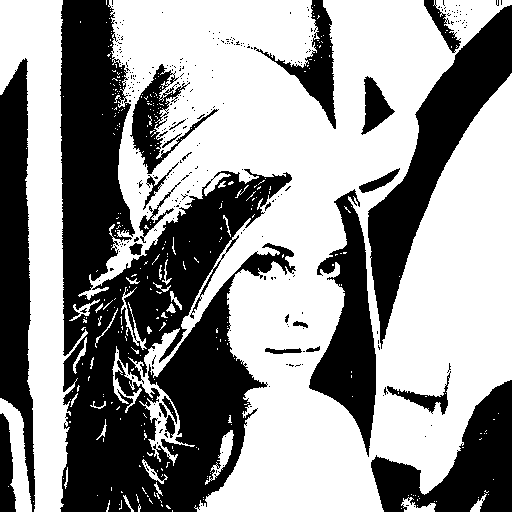
\includegraphics[width=\textwidth]{q3-lena-0002.png}
                \caption{$epsilon=0.002$. Time taken 0.16 seconds}
                \label{fig:5a}
        \end{subfigure}
        \begin{subfigure}[b]{0.25\textwidth}
                \centering
                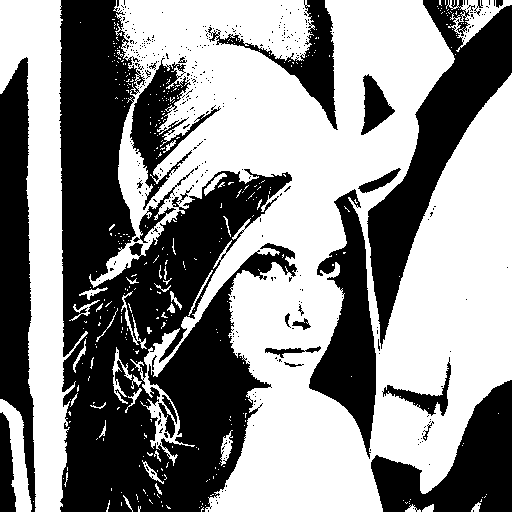
\includegraphics[width=\textwidth]{q3-lena-002.png}
                \caption{$epsilon=0.02$. Time taken 1.05 seconds}
                \label{fig:5b}
                
        \end{subfigure}
        \begin{subfigure}[b]{0.25\textwidth}
                \centering
                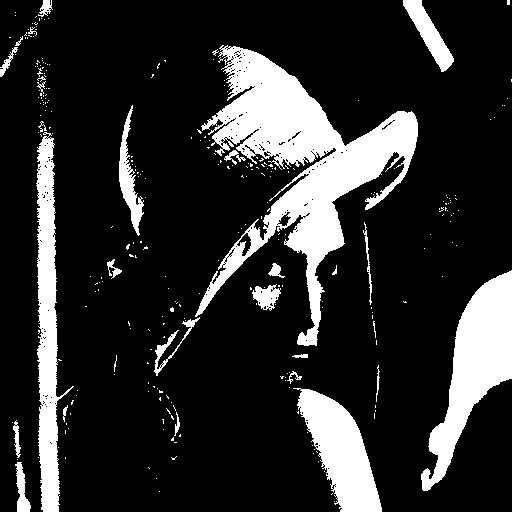
\includegraphics[width=\textwidth]{q3-lena-02.png}
                \caption{$epsilon=0.2$. Time taken 36.57 seconds}
                \label{fig:5c}
                
        \end{subfigure}
        
        \caption{Results of Double Thresholding on Lena.tif}        
        \label{fig:5}
\end{figure}

\begin{figure}[h]
    
        \centering
        \begin{subfigure}[b]{0.25\textwidth}
                \centering
                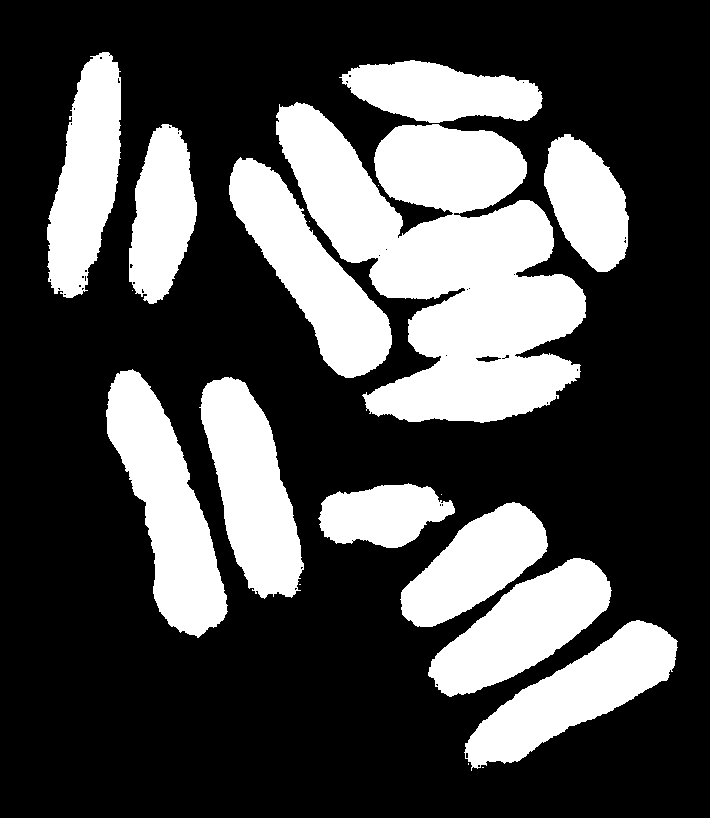
\includegraphics[width=\textwidth]{q3-yeast-001.png}
                \caption{$epsilon=0.01$.}
                \label{fig:6a}
        \end{subfigure}
        \begin{subfigure}[b]{0.25\textwidth}
                \centering
                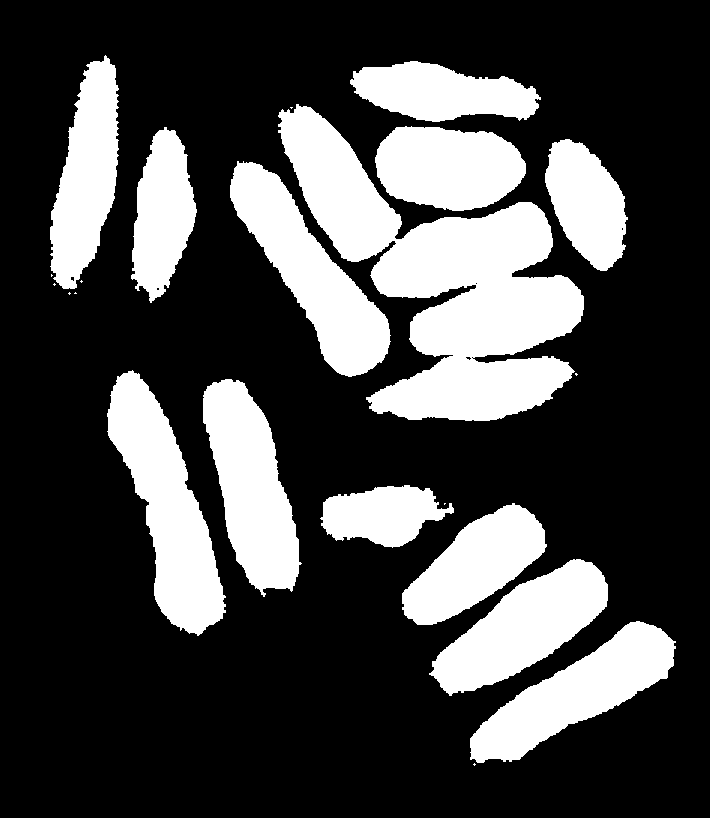
\includegraphics[width=\textwidth]{q3-yeast-002.png}
                \caption{$epsilon=0.02$. }
                \label{fig:6b}
                
        \end{subfigure}
        \begin{subfigure}[b]{0.25\textwidth}
                \centering
                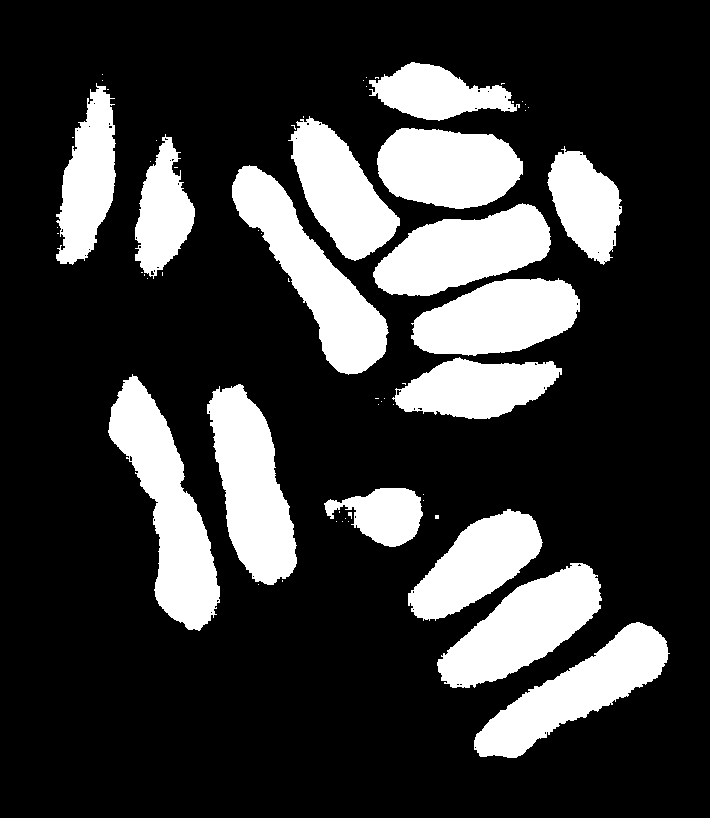
\includegraphics[width=\textwidth]{q3-yeast-004.png}
                \caption{$epsilon=0.04$.}
                \label{fig:6c}
                
        \end{subfigure}
        
        
        \caption{Results of Double Thresholding on Yeast.tif}        
        \label{fig:6}
\end{figure}
In terms of finding an other way to divide the uncertain pixels between region 1 and region 2, one option would be to determine the T1 threshold via another method than the iterative global algorithm. For example, using Otsu's method which calculates a threshold based on the histogram. I tried this, using the graythresh method in matlab (which cites Otsu's original paper in its source code). The result was almost identical to the previous one.

One could segment the image into smaller sub-images and then apply the thresholding to each subimage. This would help compensate for unevenness across the whole image. For example in the Lena image the background is not constant over the whole picture, so partitioning would potentially help the thresholding algorithm find a better local value to divide the regions (as explained in Gonzalez and Woods section 10.3.7). 

A further option would be to use a histogram matching tool (such as from the previous exercises) in order to give the input image a more `bumpy' histogram with the intensity regions better separated. This would involve first determining the correct specification histogram, then transforming the image and applying the thresholding method. I did not have time to try this approach but from reading Gonzalez and Woods I reasoned that it should be a possible solution.


A method to get rid of the `islands' of isolated pixels which occur with the double thresholding method would be to apply an object detection method to the thresholded image (for example Matlab's bwconncomp method) and then remove the smallest objects found. The bwconncomp function will give coordinates for all objects (with pixel value 1 in a binary image) which can then be removed. The following code would do this for all the objects smaller than the largest 13 (those I identified as big enough to be included):
\begin{lstlisting}
BW = thresholdedyeast; 
CC = bwconncomp(BW,4);
numPixels = cellfun(@numel ,CC.PixelIdxList); 

for k=1:(43-13)
    CC = bwconncomp(BW,4);
    numPixels = cellfun(@numel ,CC.PixelIdxList); 
    [smallest , idx] = min( numPixels ) ; 
    BW(CC.PixelIdxList{idx}) = 0;
end
\end{lstlisting}
The result is shown in figure \ref{fig:6d}.
\begin{figure}
   
            \centering
            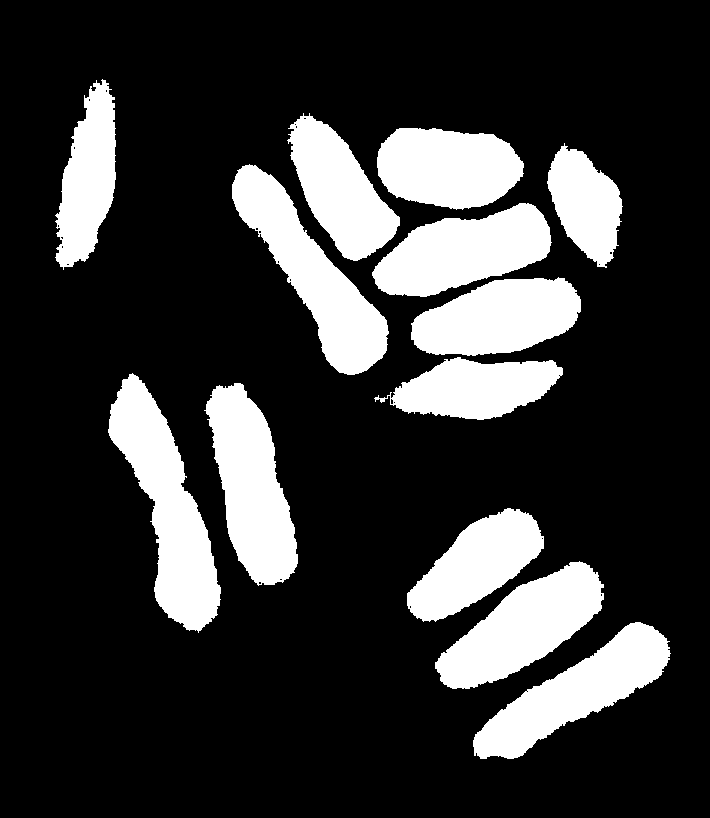
\includegraphics[width=0.4\textwidth]{q3-yeast-smallremoved-004.png}
            \caption{$epsilon=0.04$. 30 smallest objects removed}
            \label{fig:6d}
                
    
    \end{figure}
\clearpage
\appendix 
\section{edgedetector.m source} 
\label{appendix-edgedetector} 
\lstinputlisting{edgedetector.m}
\section{cannydetector.m source} 
\label{appendix-cannydetector} 
\lstinputlisting{cannydetector.m}

\section{doublethreshold.m source} 
\label{appendix-doublethreshold} 
\lstinputlisting{doublethreshold.m}

\end{document} 
